\cotefile{104}
\scanpage{2}

\figure{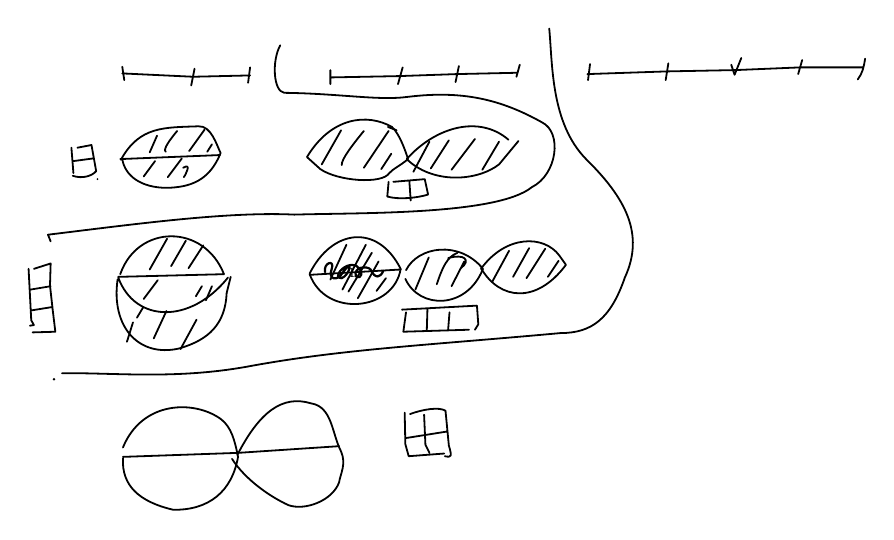
\begin{tikzpicture}[x=.0085cm,y=-.0085cm,line width=.65pt,line cap=round,line join=round]
% Three marked segments across the top.
\draw (227,131)--(333,136)--(418,134) (227,121)--(230,141) (335,124)--(330,149) (418,122)--(415,145);
\draw (538,137)--(641,135)--(727,132)--(818,130) (538,126)--(538,147) (646,122)--(639,147) (730,120)--(725,144) (821,118)--(816,136);
\draw (922,132)--(1041,128)--(1144,126)--(1240,122)--(1334,122) (926,117)--(923,141) (1043,116)--(1039,141) (1137,118)--(1142,133)--(1152,108) (1243,111)--(1237,132) (1337,109) .. controls (1335,122) and (1333,131) .. (1326,140);
% The long dividers pass between the groups of figures.
\draw (463,89) .. controls (450,113) and (453,158) .. (469,160)
 .. controls (552,161) and (610,172) .. (654,166)
 .. controls (736,156) and (793,170) .. (854,204)
 .. controls (885,219) and (877,282) .. (839,301)
 .. controls (787,343) and (583,339) .. (484,342)
 .. controls (384,337) and (240,357) .. (116,372)--(120,382);
\draw (865,64) .. controls (870,116) and (867,205) .. (920,259)
 .. controls (979,317) and (1008,371) .. (978,436)
 .. controls (957,497) and (929,519) .. (882,519)
 .. controls (685,537) and (557,543) .. (420,568)
 .. controls (309,589) and (217,578) .. (137,579);
\fill (125,588) circle[radius=2.2];
% Upright two-cell strip and bisected, hatched oval.
\draw (151,242)--(154,280) (160,242)--(181,238)--(188,277) .. controls (182,284) and (168,289) .. (153,284)
 (154,262)--(184,258);
\fill (190,289) circle[radius=1.45];
\draw (225,260) .. controls (253,209) and (291,212) .. (341,210)
 .. controls (360,209) and (368,238) .. (374,250)
 .. controls (357,292) and (328,301) .. (294,302)
 .. controls (255,302) and (231,284) .. (227,259);
\draw (224,259)--(373,253);
\draw (279,224)--(268,249) (309,217)..controls(299,229)and(287,245)..(292,248)
 (350,215)--(327,247) (361,237)--(354,248)
 (276,262)--(259,285) (316,258)--(295,286) (318,272)..controls(331,264)and(322,282)..(319,286);
% Two joined lenses, above a two-cell strip.
\draw (503,256) .. controls (539,196) and (593,190) .. (630,211)
 .. controls (641,221) and (650,246) .. (654,259)
 .. controls (641,270) and (632,273) .. (626,280)
 .. controls (615,297) and (549,292) .. (523,274)--(503,256);
\draw (637,216)--(624,211)
 (652,259) .. controls (696,210) and (761,193) .. (804,230)
 (652,259) .. controls (690,296) and (756,293) .. (790,267)--(819,232);
\draw (554,216)--(525,267) (588,217)..controls(570,239)and(554,260)..(555,268)
 (625,217)--(588,272) (629,251)--(614,274)
 (686,233)--(662,278) (715,231)--(688,273) (754,229)--(719,275) (790,233)--(765,275);
\draw (625,293)--(623,315)..controls(641,320)and(668,317)..(684,312)--(679,289)--(632,293)
 (656,292)--(658,321);
% Three-cell strip, oval and additional lower boundary.
\draw (87,423)--(91,500)--(95,507)--(89,508)
 (95,423)--(120,415)--(119,448)--(123,484)--(127,517)--(93,518)
 (90,454)--(120,449) (92,485)--(123,480);
\draw (224,431) .. controls (250,356) and (349,355) .. (379,431)
 (221,435)--(379,431)
 (221,436) .. controls (246,504) and (329,506) .. (385,436)
 (220,439) .. controls (210,509) and (251,556) .. (312,542)
 .. controls (357,529) and (381,505) .. (383,459)--(389,435);
\draw (294,378)--(268,424) (322,381)--(300,419) (348,388)--(326,422)
 (280,440)--(259,468) (346,449)--(337,464) (361,449)--(352,470)
 (258,481)--(249,496) (243,503)--(234,532) (293,486)--(274,527) (338,499)--(314,543);
% Three horizontal lenses. The first contains heavily retraced ink.
\draw (507,430) .. controls (540,364) and (608,354) .. (643,423)
 .. controls (633,486) and (531,497) .. (507,431);
\draw (507,432)--(643,424);
\draw (562,387)--(538,439) (591,387)--(556,454) (600,399)--(565,457)
 (610,412)--(579,467) (621,437)--(607,456);
\draw[line width=.8pt] (530,428)..controls(527,414)and(545,408)..(540,423)
 ..controls(534,439)and(548,443)..(557,428)..controls(573,406)and(567,432)..(555,437)
 ..controls(540,438)and(558,412)..(576,418)..controls(589,427)and(585,440)..(576,434)
 ..controls(572,420)and(593,418)..(598,424)..controls(605,439)and(613,436)..(617,426);
\node[inner sep=0pt,font=\tiny] at (570,429) {\deleted{\illegible{1}}};
\draw (651,425)..controls(669,389)and(731,380)..(766,423)
 ..controls(742,484)and(671,484)..(650,438);
\draw (685,406)--(665,454) (728,399)..controls(712,405)and(705,422)..(697,446)
 (714,407)..controls(738,400)and(749,410)..(733,422) (738,412)--(719,449);
\draw (763,423)..controls(800,372)and(857,372)..(880,403)--(890,417)
 ..controls(846,476)and(791,470)..(763,422);
\draw (805,396)--(780,442) (835,392)--(811,435) (859,393)--(831,437) (879,411)--(863,435);
\draw (645,484)--(757,478)--(759,506)--(754,514)
 (651,488)--(647,517)--(745,514) (683,484)--(682,516) (716,488)--(714,513);
% Unshaded pair with one through-line and a four-cell square.
\draw (228,690)..controls(257,619)and(336,619)..(375,648)
 ..controls(390,660)and(395,679)..(400,704)
 ..controls(391,756)and(356,784)..(303,783)
 ..controls(252,771)and(226,747)..(228,706);
\draw (399,701)..controls(432,637)and(466,611)..(509,624)
 ..controls(541,629)and(540,669)..(554,696)
 ..controls(562,715)and(553,729)..(551,742)
 ..controls(541,770)and(499,785)..(475,776)
 ..controls(447,763)and(411,738)..(391,707);
\draw (228,704)--(400,698)--(551,688);
\draw (649,638)--(650,685)--(655,703)--(708,699)
 (657,640)..controls(676,633)and(700,629)..(710,635)--(715,687)
 ..controls(720,704)and(719,705)..(709,703)
 (678,641)--(680,686)--(686,698) (650,676)--(713,666);
\end{tikzpicture}}

\[
(\text{\unsure{Ss sets}})\,\unsure{\supset|\hookleftarrow}\,
(\mathrm{Cat})\,\deleted{\unsure{\supset}}\unsure{\hookleftarrow|\leftarrow}\,
(\deleted{\unsure{\mathrm{Ord}}}\unsure{\text{Préord}|\text{PréOrd}})\,
\supset\,(\mathrm{Ord})\,\supset\,
(\deleted{\unsure{\text{Triang}}}\inserted{\text{Maquettes}})
\]

\[
\unsure{F|f}x\longrightarrow Fy
\]

\[
\underset{\smile}{x}\leq\underset{\smile}{y}
\]
% archive sheet number: 1
\scanpage{3}

\noindent\begin{minipage}[t]{.34\linewidth}
\(\checkmark\)
\diagram{\begin{tikzcd}[ampersand replacement=\&,column sep=1.5em]
{\unsure{F|\mathbb F}}_0
 \& {\unsure{\mathbb F|F}}_1 \arrow[l,shift right=.7ex,"s_1"'] \arrow[l,shift left=.7ex,"t_1"]
 \& \mathbb F_2\mathord{.} \arrow[l,shift right=.7ex,"s_2"'] \arrow[l,shift left=.7ex,"t_2"]
\end{tikzcd}}
\diagram{\begin{tikzcd}[ampersand replacement=\&,column sep=1.5em]
\mathbb F_0 \arrow[r,dash,"\sigma_1", "{\unsure{\cdot|\scriptscriptstyle >}}" description,pos=.97]
 \& {\unsure{f|F}}_1 \arrow[r,"\sigma_2"]
 \& F_2
\end{tikzcd}}
\[
\mu^{\unsure{4|1}}_1\quad\mu^2_1\quad\mu^2_2
\]
\[
\begin{aligned} &a\\ &l\\ &r\end{aligned}
\]
\end{minipage}\hfill
\begin{minipage}[t]{.64\linewidth}
\figure{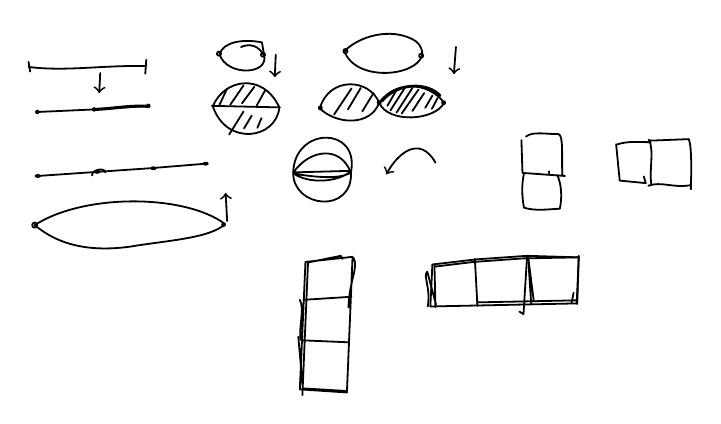
\begin{tikzpicture}[x=.0065cm,y=-.0065cm,line width=.65pt,line cap=round,line join=round]
\draw (723,94)..controls(797,103)and(858,91)..(953,92)
 (723,84)--(726,103) (953,80)--(951,107);
\draw[->] (863,106)--(861,145);
\draw (740,182)--(851,177)--(957,170);
\foreach \x/\y in {740/182,851/177,957/170}{\fill (\x,\y) circle[radius=4.4];}
\draw[line width=1.1pt] (852,177)..controls(895,175)and(917,169)..(958,171);
\draw (1096,69)..controls(1104,44)and(1144,39)..(1179,46)--(1183,70)
 ..controls(1194,110)and(1110,113)..(1096,69);
\draw (1138,55)..controls(1159,46)and(1174,56)..(1181,69);
\draw (1095,68) circle[radius=4] (1181,70) circle[radius=4];
\draw[->] (1206,70)--(1204,114);
\draw (1083,171)..controls(1105,117)and(1181,104)..(1213,173)
 ..controls(1207,235)and(1110,250)..(1083,171);
\draw (1081,170)--(1214,173);
\draw (1111,136)--(1096,168) (1143,130)--(1117,168) (1164,133)--(1140,165)
 (1185,140)--(1169,169) (1143,181)--(1115,226) (1159,189)--(1144,214) (1178,194)--(1170,213);
\draw (1340,63)..controls(1379,26)and(1443,19)..(1480,44)
 ..controls(1490,52)and(1493,63)..(1492,71)
 ..controls(1481,113)and(1362,124)..(1340,63);
\draw (1342,63) circle[radius=4] (1490,72) circle[radius=4];
\draw[->] (1558,55)--(1554,108);
\draw (1292,175)..controls(1310,112)and(1389,116)..(1408,164)
 ..controls(1391,210)and(1325,207)..(1292,175);
\draw (1408,164)..controls(1440,119)and(1504,123)..(1535,164)
 ..controls(1517,199)and(1426,205)..(1408,164);
\draw[line width=1pt] (1413,161)..controls(1445,123)and(1503,124)..(1527,150);
\foreach \x/\y in {1293/174,1408/164,1534/164}{\fill (\x,\y) circle[radius=4.8];}
\draw (1354,136)--(1320,187) (1372,135)--(1347,177) (1397,145)--(1375,181)
 (1442,139)--(1424,170) (1458,135)--(1430,179) (1473,135)--(1442,183)
 (1485,138)--(1452,185) (1496,145)--(1473,180) (1512,150)--(1498,174) (1522,155)--(1511,176);
\draw (741,307)--(857,299)--(959,292)--(1069,283);
\foreach \x/\y in {741/307,857/299,967/292,1069/283}{\fill (\x,\y) ellipse[x radius=6,y radius=3.8];}
\draw (847,306)..controls(846,294)and(873,290)..(873,300);
\draw (735,403)..controls(833,340)and(1030,343)..(1107,401)
 ..controls(1077,429)and(993,433)..(922,445)
 ..controls(814,460)and(762,425)..(735,403);
\draw (735,403) circle[radius=5];
\fill (1104,402) circle[radius=4.6];
\draw[->] (1111,395)--(1108,340);
\draw (1240,301)..controls(1242,210)and(1370,209)..(1353,299)
 ..controls(1357,382)and(1240,370)..(1240,301);
\draw (1241,299)..controls(1274,254)and(1332,248)..(1352,299)
 (1240,300)--(1352,297) (1242,303)..controls(1271,322)and(1324,320)..(1351,299)
 (1244,303)..controls(1288,310)and(1328,313)..(1350,302);
\draw[->] (1518,281)..controls(1487,226)and(1444,263)..(1422,304);
\draw (1686,237)--(1688,301)--(1771,307)
 (1695,230)..controls(1707,219)and(1739,226)..(1758,225)
 ..controls(1769,227)and(1764,273)..(1766,305)
 (1740,302)--(1740,298)
 (1691,302)..controls(1686,324)and(1687,348)..(1691,369)
 ..controls(1715,376)and(1736,372)..(1761,371)
 ..controls(1766,347)and(1764,323)..(1756,305);
\draw (1871,245)--(1878,316)--(1929,321)--(1925,308)
 (1871,246)..controls(1894,238)and(1917,241)..(1938,241)
 (1935,236)..controls(1946,257)and(1935,296)..(1940,325)
 (1937,238)--(2013,235)..controls(2019,250)and(2018,298)..(2017,333)
 (1934,326)..controls(1961,317)and(1980,331)..(2017,325);
\draw (1264,475)--(1356,465)--(1345,730)--(1253,724)--cycle
 (1260,549)--(1354,543) (1256,628)--(1348,632)
 (1258,735)--(1269,476)--(1333,463)--(1336,469)
 (1358,467)..controls(1368,486)and(1350,509)..(1348,564)
 (1253,549)..controls(1263,567)and(1250,604)..(1255,627)
 (1250,621)--(1259,722)--(1342,727);
\draw (1512,480)--(1597,470)--(1697,463)--(1798,466)--(1794,556)--(1508,562)--cycle
 (1595,469)--(1600,561) (1697,464)--(1690,577)--(1682,572);
\draw (1518,484)--(1592,475)--(1690,468)--(1799,466)
 (1503,562)..controls(1509,524)and(1493,502)..(1502,494)--(1519,558)
 (1518,563)--(1516,480) (1599,554)--(1794,550) (1705,556)--(1699,464)--(1710,551)
 (1784,555)--(1788,535) (1795,557)--(1798,463);
\end{tikzpicture}}
\end{minipage}

% printed form
% Typed address label, running from the bottom toward the top of the sheet.
\noindent\texttt{MR\quad LE PROFESSEUR GROTHENDIECK ALEX.}\\
\texttt{MATHEMATIQUES\unsure{.}\hspace{8em}5}

\[
I_A\,\unsure{\circ|:}\,\unsure{S|s|\delta}\longrightarrow S
\]

\figure{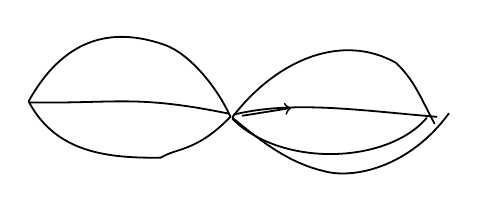
\begin{tikzpicture}[x=.014cm,y=-.014cm,line width=.65pt,line cap=round]
\draw (265,1054)..controls(300,991)and(347,988)..(389,1003)
 ..controls(411,1011)and(436,1041)..(448,1068)
 ..controls(417,1100)and(399,1096)..(385,1105)
 ..controls(329,1106)and(288,1097)..(265,1054);
\draw (266,1055)..controls(347,1056)and(362,1048)..(446,1065);
\draw (450,1068)..controls(491,1015)and(550,992)..(598,1019)
 ..controls(615,1035)and(620,1050)..(633,1074)
 (646,1065)..controls(610,1114)and(559,1125)..(532,1117)
 ..controls(498,1109)and(471,1086)..(450,1069);
\draw (451,1066)..controls(504,1053)and(564,1062)..(635,1068)
 (450,1070)..controls(494,1114)and(590,1111)..(626,1069);
\draw[->] (459,1067)--(503,1060);
\end{tikzpicture}}

\figure{\begin{tikzpicture}[x=.011cm,y=-.011cm,line width=.65pt,line cap=round]
\draw (1326,876)..controls(1346,861)and(1385,870)..(1418,869)--(1439,944)
 (1331,884)--(1345,942)..controls(1348,950)and(1384,947)..(1402,949)--(1398,943)
 (1424,859)--(1515,854)..controls(1535,874)and(1536,912)..(1538,945)
 (1408,956)..controls(1444,943)and(1500,953)..(1542,939)
 (1343,947)..controls(1346,970)and(1348,992)..(1361,1013)
 ..controls(1396,1033)and(1419,1029)..(1445,1016)--(1548,1012)--(1541,944)
 (1435,949)--(1444,1019) (1444,957)--(1445,1011) (1538,998)--(1541,1012);
\draw (1711,748)--(1725,862) (1716,713)--(1734,775)
 (1709,763)--(1843,753)--(1939,748)--(2043,744)--(2167,739)
 (1725,760)--(1834,762)
 (1838,737)--(1845,770) (1935,735)--(1942,760)
 (2041,735)--(2047,752) (2153,730)--(2153,756) (2163,735)--(2162,746);
\end{tikzpicture}}

\[
\Delta_{n_1}\times\Delta_{n_2}\times
\unsure{\mathord{-}\,\mathord{-}|\cdots}\,\unsure{\times|<}\,\Delta_{n_{\unsure{n|r}}}
\]

\figure{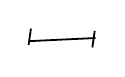
\begin{tikzpicture}[line width=.65pt]
\draw (0,0)--(.85,.04) (0,-.05)--(.03,.16) (.81,-.08)--(.84,.13);
\end{tikzpicture}}

\diagram{\begin{tikzcd}[ampersand replacement=\&,column sep=1.4em,row sep=1em,cells={nodes={inner sep=.4pt}}]
\bullet\arrow[r]\arrow[d] \& {}\arrow[r] \& {}\arrow[r] \& {}\arrow[r] \& \bullet\\
{} \& \& \& \&
\end{tikzcd}}

\[
\Delta_{n_1}\times\Delta
\]

\noindent\begin{minipage}{.40\linewidth}
\diagram{\begin{tikzcd}[ampersand replacement=\&,column sep=1.4em,row sep=1.2em,cells={nodes={inner sep=0pt,minimum size=0pt}},
 execute at end picture={\foreach \rowa/\rowb in {1/2,2/3,3/4}{
 \foreach \fracx/\fracy/\low/\high in {.04/.37/.12/.97,.24/.68/.03/.89,.62/.93/.16/.77}{
 \path (\tikzcdmatrixname-\rowb-1.center)--(\tikzcdmatrixname-\rowb-2.center) coordinate[pos=\fracx] (hatchlo);
 \path (\tikzcdmatrixname-\rowa-1.center)--(\tikzcdmatrixname-\rowa-2.center) coordinate[pos=\fracy] (hatchhi);
 \path (hatchlo)--(hatchhi) coordinate[pos=\low] (inklo) coordinate[pos=\high] (inkhi);
 \draw[line width=.33pt] (inklo)--(inkhi);}}}]
{}\arrow[r]\arrow[d,dash] \& {}\arrow[r]\arrow[d,dash] \& {}\arrow[r]\arrow[d,dash] \& {}\arrow[r]\arrow[d,dash] \& {}\arrow[d,dash]\\
{}\arrow[r]\arrow[d,dash] \& {}\arrow[r]\arrow[d,dash] \& {}\arrow[r]\arrow[d,dash] \& {}\arrow[r]\arrow[d,dash] \& {}\arrow[d,dash]\\
{}\arrow[r]\arrow[d,dash] \& {}\arrow[r]\arrow[d,dash] \& {}\arrow[r]\arrow[d,dash] \& {}\arrow[r]\arrow[d,dash] \& {}\arrow[d,dash]\\
{}\arrow[r] \& {}\arrow[r] \& {}\arrow[r] \& {}\arrow[r] \& {}
\arrow[from=1-1,to=2-2,draw=none,"\Downarrow" description]
\arrow[from=1-2,to=2-3,draw=none,"\Downarrow" description]
\arrow[from=1-3,to=2-4,draw=none,"\Downarrow" description]
\arrow[from=1-4,to=2-5,draw=none,"\Downarrow" description]
\arrow[from=2-1,to=3-2,draw=none,"\Downarrow" description]
\arrow[from=2-2,to=3-3,draw=none,"\Downarrow" description]
\arrow[from=2-3,to=3-4,draw=none,"\Downarrow" description]
\arrow[from=2-4,to=3-5,draw=none,"\Downarrow" description]
\arrow[from=3-1,to=4-2,draw=none,"\Downarrow" description]
\arrow[from=3-2,to=4-3,draw=none,"\Downarrow" description]
\arrow[from=3-3,to=4-4,draw=none,"\Downarrow" description]
\arrow[from=3-4,to=4-5,draw=none,"\Downarrow" description]
\arrow[from=1-1,to=2-1,dash,shift left=.22ex]
\arrow[from=2-1,to=3-1,dash,shift left=.22ex]
\arrow[from=3-1,to=4-1,dash,shift left=.22ex]
\arrow[from=1-2,to=4-2,dash,shift right=.3ex]
\arrow[from=1-3,to=4-3,dash,shift right=.3ex]
\arrow[from=1-4,to=4-4,dash,shift right=.3ex]

\end{tikzcd}}
\end{minipage}\hfill
\begin{minipage}{.58\linewidth}
\figure{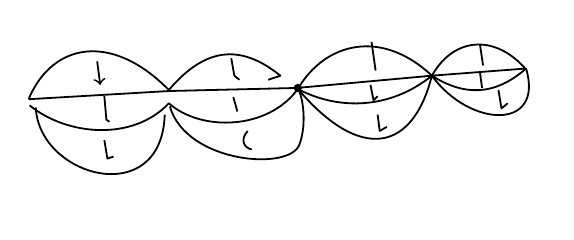
\begin{tikzpicture}[x=.013cm,y=-.013cm,line width=.65pt,line join=round]
\draw (1010,1405)..controls(1033,1350)and(1091,1339)..(1147,1396)
 ..controls(1186,1350)and(1221,1354)..(1256,1382)--(1244,1386)
 (1273,1395)..controls(1300,1349)and(1355,1336)..(1404,1382)
 ..controls(1426,1343)and(1467,1342)..(1496,1376);
\draw (1010,1405)--(1147,1397)--(1272,1394)--(1404,1382)--(1496,1375);
\draw (1011,1411)..controls(1048,1441)and(1112,1446)..(1147,1409)
 ..controls(1179,1437)and(1244,1435)..(1273,1395)
 ..controls(1313,1416)and(1363,1415)..(1404,1382)
 ..controls(1434,1401)and(1464,1403)..(1496,1375);
\draw (1017,1413)..controls(1020,1481)and(1140,1514)..(1143,1420)
 (1148,1412)..controls(1164,1468)and(1268,1476)..(1275,1448)
 ..controls(1281,1431)and(1279,1408)..(1274,1396)
 ..controls(1334,1466)and(1385,1457)..(1404,1382)
 ..controls(1441,1433)and(1514,1436)..(1496,1375);
\fill (1273,1394) circle[radius=4];
\draw[->] (1077,1368)--(1080,1391);
\draw (1084,1402)--(1086,1425)--(1089,1427) (1084,1445)--(1087,1463)--(1093,1461)
 (1208,1365)--(1211,1382)--(1216,1386) (1210,1403)--(1214,1417)
 (1224,1436)..controls(1216,1445)and(1221,1453)..(1228,1454)
 (1345,1349)--(1349,1377) (1344,1391)--(1347,1406)--(1351,1402)
 (1351,1420)--(1353,1436)--(1360,1432)
 (1451,1352)--(1454,1372) (1451,1379)--(1453,1394)
 (1469,1396)--(1472,1414)--(1478,1409);
\end{tikzpicture}}
\end{minipage}

\[
\vcenter{\hbox{
\begin{tikzpicture}[x=.85em,y=.85em,line width=.38pt,baseline]\draw (0,0)--(.59,.92)--(.82,0)--cycle;\draw (.09,.03)--(.69,.96);\end{tikzpicture}}}_n\times\vcenter{\hbox{
\begin{tikzpicture}[x=.85em,y=.85em,line width=.38pt,baseline]\draw (0,0)--(.59,.92)--(.82,0)--cycle;\draw (.09,.03)--(.69,.96);\end{tikzpicture}}}_{n'}
\]
\[
\begin{aligned}
\mathbb F_0 &= \mathrm{Ob}\,\Delta_{\unsure{kn'|n\,n'}}\\
F_1 &= \deleted{\unsure{\mathrm{Ob}\,\Delta_n|\mathrm{O}\Delta_n}}\deleted{\unsure{\mathrm{Ob}}}{\unsure{\mathbb F|F}}\mathrm{l}(\Delta_n)\times\mathrm{Ob}\,\Delta_{n'}\\
F &\mathrel{\unsure{-|=}} \mathbb F\mathrm{l}\,(\Delta_n)\times\mathrm{Fl}\,\Delta_{n''})
\end{aligned}
\]
% Lower edge cuts through the last line.
% archive sheet number: 2
\scanpage{4}

\diagram{\begin{tikzcd}[ampersand replacement=\&,column sep=1.6em,row sep=1.2ex]
\mathrm{Ob}\,C_{\unsure{4|1}}\arrow[rr,line width=.8pt]\arrow[rr,bend left=7,dash,"\deleted{\unsure{\leftarrow|{-}}}" description,pos=.52] \& \& \mathrm{Fl}_0(\unsure{C_1|C_n})\\
{\bigl(\mathrm{Fl}\,C_1\times\mathrm{Ob}\,C_2\bigr)}
 \arrow[u,shift left=.55ex]\arrow[u,shift right=.55ex]
 \& {\deleted{\unsure{\amalg}}\;\deleted{\unsure{\mathrm{Fl}_0 C_1\times}}\;
 \inserted{\unsure{\mathbb F|F}\mathrm l_0(C_1)\times\mathrm{Ob}\,C_2}} \&
\end{tikzcd}}

\[
\mathbb F\mathrm l\,C_{\deleted{\unsure{2}}\unsure{1|2}}\times
\mathrm{Fl}(C_2)\times\deleted{\unsure{\mathrm{Fl}}}\mathrm{Ob}\,C_3
\]

\figure{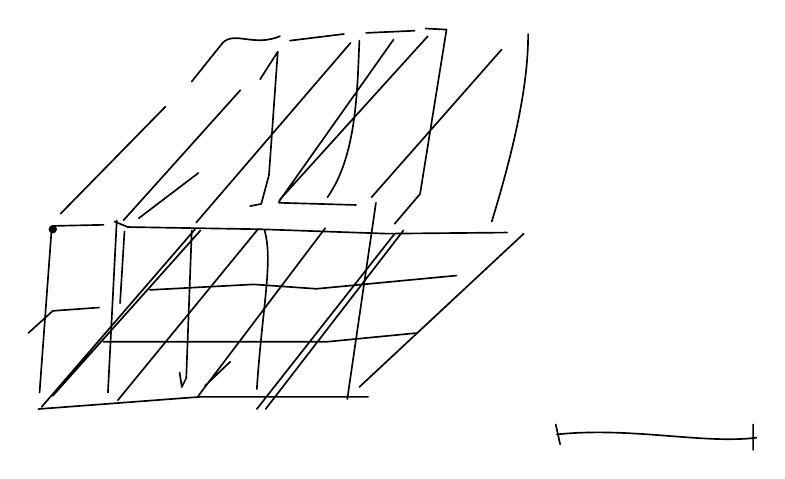
\begin{tikzpicture}[x=.014cm,y=-.014cm,line width=.6pt,line cap=round,line join=round]
\draw (1305,284)--(1351,283) (1361,280)--(1373,285)--(1493,287)--(1608,291)--(1717,290)
 (1304,286)--(1293,435) (1363,279)--(1355,435) (1370,289)--(1366,354)
 (1431,288)--(1426,422)--(1422,430)--(1420,417)
 (1497,288)..controls(1505,316)and(1495,357)..(1490,432) (1598,263)--(1572,441);
\draw (1292,450)--(1438,439)--(1591,439)
 (1295,448)--(1434,287) (1305,438)--(1439,288)
 (1364,442)--(1491,287) (1437,438)--(1552,286) (1443,429)--(1466,407)
 (1490,450)--(1615,291) (1498,450)--(1623,288) (1583,430)--(1732,291);
\draw (1283,381)--(1305,361)--(1347,358) (1351,389)--(1554,389)--(1636,381)
 (1393,342)--(1487,337)--(1544,341)--(1671,329);
\draw (1312,273)--(1407,176) (1369,279)--(1475,161) (1383,277)--(1437,236)
 (1431,153)--(1459,118)..controls(1470,107)and(1487,122)..(1511,112)
 (1493,151)--(1509,126)--(1501,238)--(1494,264)--(1484,266)
 (1520,116)--(1569,110) (1435,281)--(1575,118)
 (1510,262)--(1614,115) (1510,263)--(1580,265)
 (1554,258)..controls(1581,220)and(1581,159)..(1583,116)
 (1589,109)--(1633,107) (1511,260)--(1645,112)
 (1643,105)--(1662,106)--(1638,255)--(1615,282)
 (1594,258)--(1712,124) (1703,280)..controls(1725,208)and(1736,154)..(1736,110);
\fill (1305,287) circle[radius=3.8];
\draw (1762,473)..controls(1830,466)and(1895,482)..(1943,476)
 (1761,464)--(1765,482) (1940,464)--(1940,487);
\end{tikzpicture}}

\[
\mathbb F_3=\mathrm{Fl}\,C_1\times\mathrm{Fl}\,C_2
\,\unsure{<|\times}\,\mathrm{Fl}\,\unsure{l_3|C_3}\times\mathrm{Ob}\,C_4
\]

\[
\mathbb F_n\mathrel{\unsure{=|2}}\mathbb F\mathrm l\,C_1
\times\mathrm{Fl}\,C_2\ \text{---}\ \times\mathrm{Fl}\,C_n
\deleted{\times\mathrm{Ob}\,C_4}
\]

\figure{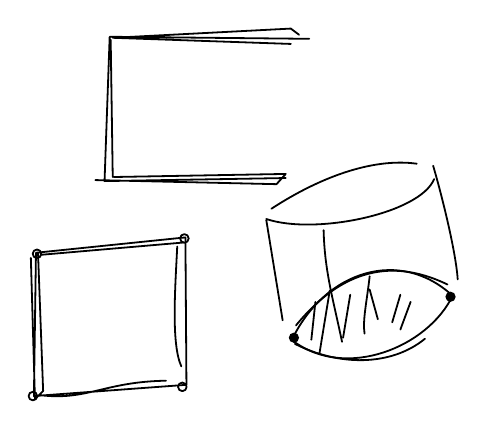
\begin{tikzpicture}[x=.013cm,y=-.013cm,line width=.65pt,line cap=round,line join=round]
\draw (1805,608)--(1610,606)--(1605,747)--(1782,744)
 (1795,604)--(1787,598)--(1613,607)--(1787,613)
 (1611,609)--(1613,743) (1596,746)--(1773,750)--(1782,740)--(1614,743);
\draw (1538,817)--(1684,802)--(1685,946)--(1536,957)--cycle
 (1543,819)--(1682,807) (1533,822)--(1537,960)--(1545,952)--(1540,817)
 (1676,811)..controls(1674,852)and(1670,906)..(1680,928)
 (1541,956)..controls(1588,962)and(1604,943)..(1665,942);
\foreach \x/\y in {1539/818,1683/803,1681/948,1535/957}{\draw (\x,\y) circle[radius=4.2];}
\draw (1768,774)..controls(1814,744)and(1866,724)..(1910,730)
 (1763,784)..controls(1810,800)and(1913,779)..(1927,745)
 (1763,785)--(1779,883) (1926,732)..controls(1932,752)and(1948,813)..(1950,843)
 (1819,795)..controls(1820,835)and(1828,861)..(1837,904);
\draw (1789,900)..controls(1822,834)and(1894,812)..(1945,859)
 ..controls(1921,909)and(1841,942)..(1789,903);
\draw (1792,888)..controls(1832,839)and(1880,819)..(1940,848)
 (1791,906)..controls(1834,928)and(1885,928)..(1918,901);
\draw (1811,865)--(1807,902) (1825,854)--(1815,915) (1845,858)--(1838,900)
 (1864,840)..controls(1861,866)and(1857,883)..(1859,896)
 (1864,853)--(1872,882) (1894,858)--(1886,885) (1904,865)--(1894,892);
\fill (1790,900) circle[radius=5] (1943,860) circle[radius=5];
\end{tikzpicture}}

\[
\tikz[baseline=(markletters.base)]{
 \node[inner sep=0pt] (markletters) {\(\unsure{X_0|X_{\varnothing}}\qquad\unsure{X_1}\)};
 \draw[line width=.32pt] ([xshift=.29em,yshift=-.28em]markletters.west)
 ..controls ([xshift=1.5em,yshift=-.75em]markletters.west) and ([xshift=-1.65em,yshift=.40em]markletters.east)
 ..([xshift=-.63em,yshift=.06em]markletters.east);}
\]

\[
\bullet\quad O_1\subset F_1\qquad
\deleted{\mathbb F}O_2\subset\mathbb F_2\quad\text{---}\quad O_n\subset F_n
\]

\[
\deleted{O}\unsure{\dot F|\hat F}\subset F
\]

\[
\mathbb F_1\times\text{---}\ \times\mathbb F_n\times(\unsure{-}\,?)
\]

\[
(O_1,F_1)\mathbin{*}(O_2,\mathbb F_2)\ \text{---}\mathbin{*}
(\deleted{\unsure{O|0}}\unsure{O_3|O_n}\,\unsure{F_n|F_3})\,.
\]

\figure{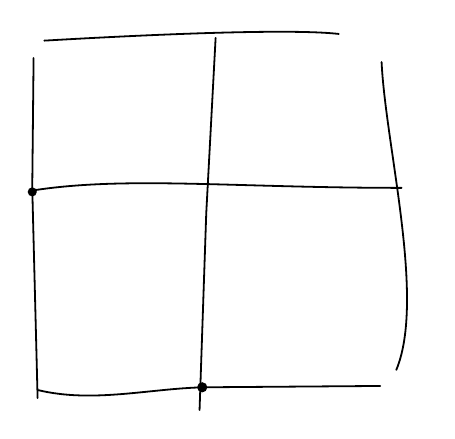
\begin{tikzpicture}[x=.017cm,y=-.017cm,line width=.65pt,line cap=round]
\draw (1374,1202)..controls(1460,1197)and(1559,1193)..(1594,1197)
 (1366,1215)--(1365,1312)--(1369,1469)
 (1365,1314)..controls(1435,1303)and(1515,1312)..(1641,1312)
 (1502,1200)--(1495,1331)--(1490,1478)
 (1369,1463)..controls(1410,1473)and(1452,1462)..(1493,1461)--(1625,1460)
 (1626,1218)..controls(1629,1281)and(1659,1395)..(1637,1448);
\fill (1365,1315) circle[radius=3.4] (1492,1461) circle[radius=3.8];
\end{tikzpicture}}

\[
(F\times I)\mathbin{\amalg}_{\deleted{O}\dot F\times I}\deleted{O}\dot F
\]
% archive sheet number: 3
\scanpage{5}

\diagram{\begin{tikzcd}[ampersand replacement=\&,column sep=1.4em]
{\mathbb Z[\unsure{\mathbb F|F}_{\unsure{n-2|n\,2}}]}
 \& {\mathbb Z[\mathbb F_{n-1}]}\arrow[l]
 \& {\mathbb Z[F_n]}\arrow[l,"{t_n-s_n}"]
 \& {\mathbb Z[\mathbb F_{n+1}]}\arrow[l] \& \unsure{\cdot|\text{,}}
\end{tikzcd}}

\[
\begin{aligned}
D_n&\longrightarrow X &\quad&\deleted{D_n}\unsure{.}\\
\bigl\{x&\in F_n && =\\
t_{n-1}{}&
\underset{\substack{\unsure{E_3}\hfill\\0}}{\underbrace{\vphantom{\bigg|}\bigl(t_n\unsure{(f)|f)}-s_n(f)\bigr)}}
-s_{n-1}\bigl(t_n(f)-s_n\unsure{(f)|f)}\bigr)&&
\end{aligned}
\]

\[
\begin{array}{cc}
\underset{\smile}{F}_0 & F_1\\[.6em]
F'_0 & \mathbb F'_1\\
\unsure{\prime|1}&
\end{array}
\]
\diagram{\begin{tikzcd}[ampersand replacement=\&,column sep=1.7em,row sep=1.3ex]
\&\& \unsure{s}\&\unsure{t}\arrow[l]\\
{\substack{\exists\,\deleted{\unsure{u}}s,u'\\s'}} \&
 f(s)\arrow[l] \& f_0(s) \& f_0(t)\arrow[l]
\end{tikzcd}}

\begin{flushright}
\begin{minipage}{.74\linewidth}
\(\bigl(C_i\bigr)\quad\forall w'\in F'_i,\)
\deleted{si on \unsure{retient|retire|choisit}} \(\deleted{\unsure{s}}\exists w\in\mathbb F_i\) tel que
\(f(w)\sim w'\). De plus si \(i\geq1\), On peut
\par\noindent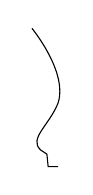
\begin{tikzpicture}[baseline=-2.3em,x=.45em,y=.5em,line width=.4pt]
\draw (0,5)..controls(1.7,3)and(2.6,1)..(2.1,-.4)
 ..controls(1.4,-2)and(-.3,-3)..(.7,-3.8)--(1.2,-4.1)--(1.3,-5)--(2.1,-5);
\end{tikzpicture}\begin{minipage}{.89\linewidth}
se \unsure{donner}
d'avance \(u_{i\unsure{-1}}=s_i(w)\), \inserted{\(v_{i\unsure{-1}}=\)}\(t_i(w)\),
\inserted{\unsure{de|dans} \(F_{i-1}\),} soumis aux seules conditions \deleted{\unsure{de}} que
\(f(u_{\unsure{i|1}})=u'_{\unsure{i|1}}\), \inserted{\(\unsure{\text{resp}}\)}
\(\unsure{g|f}(v_{\unsure{i|1}})=v'_{\unsure{i|1}}\)
et, \deleted{de} plus, si \(i-1\geq1\) i.e \(i\geq2\), \deleted{\unsure{que}}
\(s(u)=s(v),\ t(u)=t(v)\)
\end{minipage}

(\unsure{NB} on n'exige pas que \(\unsure{g|f}(u)=u'\))
\end{minipage}
\end{flushright}

\[
\begin{aligned}
\unsure{E|\Xi}_0\quad\text{\textcircled{\(\unsure{\mathrm a)|\mathrm b)}\)}}\quad&
\forall s'\in F'_0,\quad \exists s\in F_0,\ u\in F'_1,\quad
f_0(s)\xrightarrow{u}s'\\[-.1em]
&\hspace{4em}\deleted{\pi_0(f)\ \unsure{\text{surj}}}\quad
\unsure{-}\pi_0(f)\ \text{\uuline{\unsure{surj}}}\\
\mathrm b)\quad&
\forall s,t\in F_0,\quad
\underset{\substack{\rotatebox{90}{\(\in\)}\\F'_1}}{u'}:f_0(s)\longrightarrow f_0(t),\\
&\exists u\in\mathbb F_1,\quad u:s\mathbin{-}t\qquad\pi_0(f)\ \text{inj.}
\end{aligned}
\]

\[
\begin{aligned}
E_1\quad\text{\textcircled{\(\mathrm b')\)}}\quad&
\forall s,t\in F_0,\quad
\underset{\substack{\rotatebox{90}{\(\in\)}\\F'_1}}{u'}:
 f_0(s)\mathbin{-} f_0(t),\\
&\exists u\in F_1,\quad u:s\mathbin{-}t,\quad
 f(u)\xrightarrow[\sim]{\unsure{\epsilon|\ell}}u'\\
&\deleted{\unsure{\exists\,w\in F_2}}\\
&\pi_0(f)\ \text{inj. et }\text{\uuline{\(\pi_1(f)\) surj}}
\end{aligned}
\]

\[
\begin{aligned}
\mathrm c)\quad&
\deleted{\forall s,t\in\unsure{\mathbb F_0},}\ u,v\in F_1\quad
\begin{gathered}s_{\unsure{i|1}}(u)=s_1(v),\\[-.2em] t_1(u)=t_1(v)\end{gathered},\\
&\text{et }\underset{\substack{\rotatebox{90}{\(\in\)}\\F'_2}}{w'}:
 f(u)\longrightarrow f(v),\quad
 \exists\underset{\substack{\rotatebox{90}{\(\in\)}\\F_2}}{w}:
 \deleted{\unsure{f|f_1}}u\mathbin{-}v\\
&\pi_{\unsure{1|f}}(f)\ \text{inj.}
\end{aligned}
\]
\diagram{\begin{tikzcd}[ampersand replacement=\&,column sep=2.4em,cells={nodes={inner sep=0pt}}]
{}\arrow[r,bend left=45,"u"]\arrow[r,bend right=45,"v"']\&{}
\end{tikzcd}}

\[
\begin{aligned}
E_2\quad\text{\textcircled{\(\mathrm c'\)}}\quad&
\forall(u,v)\in F_1,\quad
\begin{gathered}s_1(u)=s_1(v)\\[-.2em] t_1(u)=t_1(v)\end{gathered}
\quad\text{et }\underset{\substack{\rotatebox{90}{\(\in\)}\\F'_2}}{w'}:
 f(u)\mathbin{-}f(v),\\
&\exists\underset{\substack{\rotatebox{90}{\(\in\)}\\F_2}}{w}:u\longrightarrow v\
 \deleted{\unsure{et|f}}\ \text{tel que}\\
&w'\sim f(w)\qquad\overbrace{\pi_1(f)\ \text{inj et }\pi_2(f)\ \text{surj}}
\end{aligned}
\]
\diagram{\begin{tikzcd}[ampersand replacement=\&,column sep=1.7em,cells={nodes={inner sep=0pt}}]
{}\arrow[r,bend left=46,dash,"{f(u)}"]\arrow[r,bend right=42,dash]
 \arrow[r,draw=none,"{w'\!\downarrow}" description]\&{}
\end{tikzcd}}
% archive sheet number: 4
\scanpage{6}

% Typed slip, running from the bottom toward the top at left.
\[
\underline{\mathrm B}=(\text{Gr-stacks})\qquad
\widehat{\underline{\mathrm B}}\qquad
\underline{\mathrm B}(\unsure{0|\mathrm O})^{\wedge}
\]
commutes not only with arbitrary projective limits, but equally with arbitrary direct limits, or what amountsto the same, that direct limits in the category (Gr-stacks) can be computed component-wise. (Here \(\underline{\mathrm B}(0)\) stands for the full subcategory of \(\underline{\mathrm B}\) formed by the basic objects \(\underline{\mathrm D}_n\), \(n\ \underline{\mathrm N}\) .)

\[
\widetilde{\unsure{D|\mathbb D}}\qquad
\unsure{N|\mathscr N}\longmapsto
\overset{\deleted{\unsure{I_n|D_n}}}{\widetilde D_n}
\]

\[
\begin{aligned}
&1+n\mathbin{.}2^1+\frac{n(n-1)}{2}\,2^2\ \text{---}\ +2^n\\
&\qquad=(1+2)^n=
\end{aligned}
\]

\diagram{\begin{tikzcd}[ampersand replacement=\&,row sep=1.15em,column sep=2em]
\widetilde D_{n'}\arrow[r,bend left=38]\arrow[r]\arrow[r,bend right=38]\&
\widetilde D_n\\
\&\widetilde D_n\arrow[d]\\
\&n\in{\unsure{\mathbb I|I}}
\end{tikzcd}}
\[
\begin{aligned}
d_n\in\widetilde D_n&\longrightarrow\deleted{\unsure{N}}\mathbb I
 &\qquad d_n&\longmapsto n\\
&\text{strictement}\\
&\text{\unsure{croissante}}\\
&\text{image \unsure{est|\(=\)|\(\subset\)}}\ \mathbb I_{\deleted{\unsure{\in n}}\leq n}
\end{aligned}
\]

% margin note written sideways
\margin{\resizebox{.99\marginparwidth}{!}{\begin{minipage}{17em}
\diagram{\begin{tikzcd}[ampersand replacement=\&,column sep=1.3em,row sep=.65em]
{\unsure{J|I}_{n''}}\arrow[r,"{\unsure{u_\eta|u_g|u_y}}"] \&
 {\overset{\substack{\unsure{\eta|y}\\\rotatebox{90}{\(\in\)}}}{J}_{n'}}
 \arrow[r,"{\overset{\deleted{\unsure{u_\eta|u_g}}}{\unsure{u_\xi|u_f}}}"]
 \arrow[dr,bend right=16,sloped,"\unsure{u}"'] \&
 {\overset{\substack{\unsure{\xi|x}\\\rotatebox{90}{\(\in\)}}}{J}_{\deleted{\unsure{n'}}n}}\\
 \& \& \unsure{\xi|x|f}
\end{tikzcd}}
\(u_\xi u_\eta=\)
\end{minipage}}}

\[
\widetilde D_{n'}\longrightarrow\widetilde D_n
\]
\diagram{\begin{tikzcd}[ampersand replacement=\&,column sep=1.25em,row sep=.8em]
x''\arrow[d,dash,"\deleted{\unsure{=}}"'] \& {<} \& x'\arrow[d,dash] \& {\in} \& {\overset{\deleted{\unsure{D}}}{\widetilde D_n}}\\
y'' \& {<} \& y'\arrow[d,dash] \& {\in} \& {}\\
n'' \& \& n' \& \&
\end{tikzcd}}
\figure{\begin{tikzpicture}[line width=.6pt]
\draw (0,.75)..controls(.8,.52)and(.7,-.3)..(1.25,-.48)
 (.03,.32)..controls(.48,.08)and(.37,-.5)..(1.04,-.64);
\fill (2.7,-.48) circle[radius=.04] (2.7,-.88) circle[radius=.04];
\end{tikzpicture}}

\(I\) \unsure{ens} ordonné

\(n\longmapsto\widetilde D_n\) \unsure{famille|échelle} d'ens \unsure{ordonnés} ,

\[
\widetilde D_n\xrightarrow{\deleted{\unsure{\phi}}\unsure{k_n|\kappa_n|\tau_n}}I\qquad
\text{str. croiss.}\quad\text{image}\quad I_{\leq n}
\]

Si \(n'\leq n\), \deleted{\unsure{Soit|Sinon} l'ens \(\unsure{K}\)} Soit
\[
\begin{gathered}
\unsure{\mathscr L|\Phi|L}_{n',n}\subset\widetilde D_n\\[-.2em]
\rotatebox{90}{\(=\)}\\[-.2em]
\bigl\{x\in\widetilde D_n\mid \unsure{k_n|\kappa_n|\tau_n}(x)=n'\bigr\}
\end{gathered}
\]

\deleted{Soit \(x\in\mathscr L_{\unsure{n'}},\)}

\unsure{Considérons} l'ens \deleted{\(\unsure{\widetilde D_{n'}|D_n}\)}\(\unsure{B|\mathscr B}\)

\diagram{\begin{tikzcd}[ampersand replacement=\&,column sep=2.3em]
F_0 \& \mathbb F_1\arrow[l,shift left=.6ex]\arrow[l,shift right=.6ex]
 \& F_2\arrow[l,shift left=.6ex]\arrow[l,shift right=.6ex]
\end{tikzcd}}
\diagram{\begin{tikzcd}[ampersand replacement=\&,column sep=1em]
x\arrow[loop right,distance=2em,in=35,out=-35] \& {}
\end{tikzcd}}
\diagram{\begin{tikzcd}[ampersand replacement=\&,row sep=1.1em]
x'\arrow[d,dash]\\ y'
\end{tikzcd}}
\figure{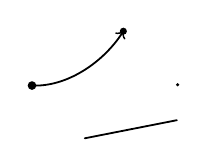
\begin{tikzpicture}[line width=.65pt,line cap=round]
\fill (0,.15) circle[radius=.055];
\draw[->] (0,.15)..controls(.45,.13)and(.91,.45)..(1.16,.84);
\fill (1.16,.84) circle[radius=.045] (1.85,.16) circle[radius=.022];
\draw (.67,-.52)--(1.84,-.29);
\end{tikzpicture}}

\[
\begin{aligned}
\pi_0(F_{\unsure{*|x}},x)&=\text{\unsure{ens} des \unsure{classes} d'\unsure{hom.topie|homotopie} des}\\
&\phantom{=}\text{\unsure{lacets} en }x
\end{aligned}
\]
% archive sheet number: 5
\scanpage{7}
\mspage{1}

Soit \(M\) une catégorie (``\unsure{modèles|modeles|modéles}''). On suppose

(i) Toute flèche de \(M\) est \unsure{monomorphique}

(ii) Tout \deleted{\unsure{autom|autom.}}\inserted{end} d'un élément de \(M\) est l'identité.

Ex : \(M\) une catégorie définie \unsure{par} un ensemble ordonné

Pour tout \(D\in\mathrm{Ob}\,M\), soit \(\widetilde D\) l'ensemble (ordonné par ``inclusion'') des sous objets de \(D\). On identifie \(D\) au plus grand élément de \(\widetilde D\)

Soient \(D',D\in\mathrm{Ob}\,M\), alors l'application
\begingroup\makeatletter\tagsleft@true\makeatother
\[
\begin{aligned}
\underset{M}{\mathrm{Hom}}(D',D)&\longrightarrow\widetilde D\\
u&\longmapsto u(D')
\end{aligned}
\tag*{(\(\ast\))}
\]
\endgroup
est injective par \unsure{(i)|[i]}(ii), son image est formée de l'ens \deleted{\unsure{de}}
\(\underset{\inserted{M}}{\unsure{\mathscr L|\Phi|L}}_{D'}(D)\subset\widetilde D\)
des sous-objets \(\Delta\) de \(D\) qui sont isomorphes à \(D'\).

\deleted{Soit \(K\) un ens. ordonné}

Soit \(N\)\deleted{\(\unsure{I|K}\)} l'ens \inserted{préordonné} des \unsure{classes} d'isom. d'objets de \(M\). \inserted{Il est en fait \uline{ordonné}, \unsure{grâce} à (ii).}
Pour \(\unsure{\forall|\mathrm H}\ n\in\unsure{\mathbb N|N}\), un\deleted{\unsure{e}} objet \(D_n\) de \deleted{\(D\)}\(M\) de classe \(\overset{\unsure{\ast|\prime}}{n}\) est déterminé à isom unique près, \unsure{à} cause de (ii), donc l'ens ordonné \(\widetilde D_n=\unsure{\mathbb J|\mathbb I}_n\) est \unsure{défini} à isom unique près. On a donc \deleted{\unsure{plus|choisi}, une}\inserted{une} \unsure{famille}
\[
(\mathbb J_n)_{n\in\mathbb N}
\]
d'ens ordonnés, \unsure{indexés} par l'ensemble ordonné \(\mathbb N\).
% archive sheet number: 6
\scanpage{8}
De plus, se rappelant la \unsure{definition|définition} de
\[
 J_n=\widetilde D_n=\text{ens des \unsure{sous-objet|sous-objets} de }D_n
\]
on a, pour \(\forall n\in\mathbb N\), une application canonique, strictement croissante
\[
 J_n\xrightarrow{\tau_n}\mathbb N \qquad\qquad
 \text{\(\tau_n\), application ``type}
\]
dont l'image est \unsure{formée|formé} \deleted{des} de l'ens
\deleted{\(I_{\leq n}\) des} \(\mathbb N_{\leq n}=\{n'\in\mathbb N\mid n'\leq n\}\).

Notons que chaque \(J_n\) a un plus grand élément, qui est ``\(D_n\) (\unsure{en tant|en} que \inserted{le} sous-objet maximal de \(D_n\)), et qu'\deleted{\unsure{est|il}}\unsure{on|on y} note \(d_n\). On a donc \inserted{(par (ii))}
\[
 \tau_n^{-1}(n)=\{d_n\}
\]
\deleted{Si \(n'\leq n\), alors pour tout \(x\in J_n\).}

Soient \(n,n'\in\mathbb N\), \deleted{\(\unsure{x\in J|x\in}\)}\deleted{\(x\in J_n,\ n'=\tau_n(x)\), on} \inserted{avec \(n'\leq n\)}
\unsure{considérons|considérer} \deleted{\unsure{via \(x\)|via \((x)\)|l'in}} \deleted{on a alors \unsure{une|un} application}
\[
 \begin{aligned}
 \mathrm{Hom}(\deleted{\unsure{O|D}}D_{n'},\unsure{D|\mathbb D}_n)&\hookrightarrow \widetilde D_n=J_n\\
 u&\longmapsto u(d_{n'})
 \end{aligned}
\]
qui est une bijection des \(\mathrm{Hom}\) sur l'ens \(\tau_n^{-1}(n')\), et considérons
\[
 \mathrm{Hom}(\deleted{\unsure{D|O}}D_{n'}^{\unsure{\ast|\prime}},D_n)
 \longrightarrow
 \mathrm{Hom}\bigl(\underset{\substack{\tikz{\draw(0,.08)--(0,0)--(.60,0)--(.60,.08);}\\ J_{n'}}}{\widetilde D_{n'}},\underset{\substack{\tikz{\draw(0,.08)--(0,0)--(.54,0)--(.54,.08);}\\J_n}}{\widetilde D_n}\bigr)
\]
on en déduit une \deleted{\unsure{bi ce|bi se}} application
\[
 \begin{aligned}
 \underset{\substack{\rotatebox{90}{\(=\)}\\ {[\mathrm{Hom}(D_{n'},D_n)]}}}{\tau_n^{-1}(n')}
 &\overset{\mathrm{def}}{=}
 \underset{\substack{\tikz{\draw(0,.07)--(0,0)--(.86,0)--(.86,.07);}\\\text{ens des}\\\text{éléments}\\\text{de \(J_n\) de}\\\text{type \(n'\)}}}{J_{n',n}\deleted{\unsure{(n')|(n)}}}
 \xrightarrow{\rho_{n,n'}}\mathrm{Hom}(J_{n'},J_n)\\
 &\hspace{7em}\text{\unsure{ou|où}}\quad \xi\longmapsto u_{\xi}^{n}
 \end{aligned}
\]
qui est injective, plus précisément on a la \unsure{commutativité|commutativite}
\diagram{\begin{tikzcd}[ampersand replacement=\&,column sep=large,execute at end picture={
 \draw ([xshift=.25em,yshift=-.15em]\tikzcdmatrixname-1-1.south east)
 ..controls +(-1.1em,.6em) and +(-2.1em,0)..
 node[pos=.95,above,inner sep=.5pt,fill=white] {\(\scriptstyle\text{inclusion}\)}
 ([xshift=.45em,yshift=-1.45em]\tikzcdmatrixname-1-2.south)
 ..controls +(1.9em,-.04em) and +(-1.0em,-.60em)..(\tikzcdmatrixname-1-3.south west);}]
 J_{n,n'} \arrow[r,"\rho_{n,n'}"]
 \& \mathrm{Hom}(J_{n'},J_n) \arrow[r,"u\mapsto u(d_{n'})"] \& J_n
\end{tikzcd}}
% archive sheet number: 7
\scanpage{9}
\mspage{2}
i.e. on a, pour \(\deleted{x}\xi\in J_n(n')\) i.e. \(x\in J_n,\ \tau_n(x)=n'\)
\[
 u_\xi(d_{n'})=\xi .
\]
\deleted{De} \unsure{plus,|\deleted{plus,}} \unsure{fort|faut|fut} encore, \(\underbrace{\text{on a :}}\) \inserted{\(u_\xi\) induit un \unsure{isom|iso}} \(J_{n'}\xrightarrow{\overset{u_\xi}{\sim}}(J_n)_{\leq\xi}\)

Lorsque \(\unsure{n'|n}=n\), on a \(J_{n,n}=\{d_n\}\), et
\[
 u_{d_n}=\mathrm{id}_{J_n}
\]

La connaissance de \(\mathbb N,\ (J_n)_{n\in\mathbb N},\ (\tau_n)_{n\in\mathbb N},\
(\rho_{n,n'})_{\substack{(n',\deleted{\unsure{n'|m}}n)\in\mathbb N\times\mathbb N\\ n'\leq n}}\) permet de reconstituer \deleted{à peu de \unsure{chose|choses} près} \deleted{essentiellement \unsure{la|le} sous-catégorie pleine}\inserted{la catégorie} \(M\), à \deleted{\unsure{il|à}} \unsure{équiv|équiva} près, il manque encore une \deleted{\unsure{description|descripteur}} \inserted{condition} pour composer les hom ``\unsure{standart|standard} entre les \(J_n\), i.e ceux provenant des \(J_{n',\unsure{n|n'}}\). \deleted{\unsure{Donc|Don}} On considère une situation
\diagram{\begin{tikzcd}[ampersand replacement=\&,column sep=.8em,row sep=small]
 \& \& \eta \& \& \xi\\[-.8em]
 \& \& \rotatebox{90}{\(\in\)} \& \& \rotatebox{90}{\(\in\)}\\
 J_{n''}\arrow[rr,"u^{n'}_{\eta}"] \& \& J_{n'}\arrow[rr,"u_\xi^n"] \& \& J_n\\
 n'' \& \leq \& n' \& \leq \& n
\end{tikzcd}}
on doit avoir
\[
 u_\xi^n\,u_\eta^{n'}=u_{\deleted{\unsure{\xi|a}}\zeta}^{n}
 \qquad\text{où}\quad \zeta=u_\xi^n(\eta)=
 (u_\xi^n\,u_\eta^{n'})(d_{n''})
\]
qui exprime la \deleted{\unsure{stabilité|composition|stabilis}} stabilité de la notion d'hom admissible \unsure{entre|entre.} \(J_n\) par composition.

\deleted{Il est évident que la \unsure{catég|caté}} \inserted{Soit \(M_0\) la catégorie définie par}
\[
 \mathrm{Ob}\,M_0=\mathbb N,\quad \mathrm{Hom}_{M_0}(n',n)=
 \left\{\begin{aligned}
 &\varnothing\ \text{si }n'\nleq n\\
 &\text{ens. des hom. admissibles}\\
 &\qquad J_{n'}\to J_n\quad\text{si }n'\leq n
 \end{aligned}\right.
\]
% archive sheet number: 8
